% Options for packages loaded elsewhere
\PassOptionsToPackage{unicode}{hyperref}
\PassOptionsToPackage{hyphens}{url}
%
\documentclass[
  12pt,
  openany]{book}
\usepackage{lmodern}
\usepackage{setspace}
\usepackage{amsmath}
\usepackage{ifxetex,ifluatex}
\ifnum 0\ifxetex 1\fi\ifluatex 1\fi=0 % if pdftex
  \usepackage[T1]{fontenc}
  \usepackage[utf8]{inputenc}
  \usepackage{textcomp} % provide euro and other symbols
  \usepackage{amssymb}
\else % if luatex or xetex
  \usepackage{unicode-math}
  \defaultfontfeatures{Scale=MatchLowercase}
  \defaultfontfeatures[\rmfamily]{Ligatures=TeX,Scale=1}
\fi
% Use upquote if available, for straight quotes in verbatim environments
\IfFileExists{upquote.sty}{\usepackage{upquote}}{}
\IfFileExists{microtype.sty}{% use microtype if available
  \usepackage[]{microtype}
  \UseMicrotypeSet[protrusion]{basicmath} % disable protrusion for tt fonts
}{}
\makeatletter
\@ifundefined{KOMAClassName}{% if non-KOMA class
  \IfFileExists{parskip.sty}{%
    \usepackage{parskip}
  }{% else
    \setlength{\parindent}{0pt}
    \setlength{\parskip}{6pt plus 2pt minus 1pt}}
}{% if KOMA class
  \KOMAoptions{parskip=half}}
\makeatother
\usepackage{xcolor}
\IfFileExists{xurl.sty}{\usepackage{xurl}}{} % add URL line breaks if available
\IfFileExists{bookmark.sty}{\usepackage{bookmark}}{\usepackage{hyperref}}
\hypersetup{
  hidelinks,
  pdfcreator={LaTeX via pandoc}}
\urlstyle{same} % disable monospaced font for URLs
\usepackage[left=4cm, right=3cm, top=3cm, bottom=3cm]{geometry}
\usepackage{longtable,booktabs}
\usepackage{calc} % for calculating minipage widths
% Correct order of tables after \paragraph or \subparagraph
\usepackage{etoolbox}
\makeatletter
\patchcmd\longtable{\par}{\if@noskipsec\mbox{}\fi\par}{}{}
\makeatother
% Allow footnotes in longtable head/foot
\IfFileExists{footnotehyper.sty}{\usepackage{footnotehyper}}{\usepackage{footnote}}
\makesavenoteenv{longtable}
\usepackage{graphicx}
\makeatletter
\def\maxwidth{\ifdim\Gin@nat@width>\linewidth\linewidth\else\Gin@nat@width\fi}
\def\maxheight{\ifdim\Gin@nat@height>\textheight\textheight\else\Gin@nat@height\fi}
\makeatother
% Scale images if necessary, so that they will not overflow the page
% margins by default, and it is still possible to overwrite the defaults
% using explicit options in \includegraphics[width, height, ...]{}
\setkeys{Gin}{width=\maxwidth,height=\maxheight,keepaspectratio}
% Set default figure placement to htbp
\makeatletter
\def\fps@figure{htbp}
\makeatother
\setlength{\emergencystretch}{3em} % prevent overfull lines
\providecommand{\tightlist}{%
  \setlength{\itemsep}{0pt}\setlength{\parskip}{0pt}}
\setcounter{secnumdepth}{4}
\usepackage[none]{hyphenat}
\usepackage[cmyk]{xcolor} % Recommended by US-AB
\usepackage{lmodern} % Recommended by US-AB
\usepackage{fancyhdr}
\usepackage{etoolbox}
\patchcmd{\chapter}{\thispagestyle{plain}}{\thispagestyle{fancy}}{}{} % Removes plain pagestyle from chapter headings (otherwise, page numbers are centered)
\AtBeginDocument{\addtocontents{toc}{\protect\thispagestyle{empty}}} 
\pagestyle{empty} % This makes ToC without header/footer
\usepackage[skip=15pt]{caption} % This should increase space below captions (not tested)
\raggedbottom
\usepackage[noindentafter]{titlesec}
\usepackage{titlesec}
\titleformat{\chapter}{\normalfont\bfseries}{\thechapter.}{15pt}{}\titlespacing*{\chapter}{0pt}{-50pt}{0pt}
\titleformat{\section}{\normalfont\bfseries}{\thesection.}{1em}{}\titlespacing*{\section}{0pt}{0pt}{0pt}
\titleformat{\subsection}[runin]{\normalfont\bfseries}{\thesubsection.}{1em}{}

\usepackage{CJKutf8} % For Mandarin in Acknowledgments

% For guiding quote in beginning of intro:
\makeatletter
% \renewcommand{\@chapapp}{}% Not necessary...
\newenvironment{chapquote}[2][2em]
  {\setlength{\@tempdima}{#1}%
   \def\chapquote@author{#2}%
   \parshape 1 \@tempdima \dimexpr\textwidth-2\@tempdima\relax%
   \itshape}
  {\par\normalfont\hfill--\ \chapquote@author\hspace*{\@tempdima}\par\bigskip}
\makeatother
\usepackage{placeins}
\usepackage{titlesec}
\newcommand{\sectionbreak}{\clearpage}
\usepackage{amsmath}
\usepackage{wrapfig}
\usepackage{caption}
\captionsetup[figure]{font=scriptsize}
\usepackage{float}
\usepackage{amssymb}
\usepackage{subcaption}
\ifluatex
  \usepackage{selnolig}  % disable illegal ligatures
\fi
\newlength{\cslhangindent}
\setlength{\cslhangindent}{1.5em}
\newlength{\csllabelwidth}
\setlength{\csllabelwidth}{3em}
\newenvironment{CSLReferences}[2] % #1 hanging-ident, #2 entry spacing
 {% don't indent paragraphs
  \setlength{\parindent}{0pt}
  % turn on hanging indent if param 1 is 1
  \ifodd #1 \everypar{\setlength{\hangindent}{\cslhangindent}}\ignorespaces\fi
  % set entry spacing
  \ifnum #2 > 0
  \setlength{\parskip}{#2\baselineskip}
  \fi
 }%
 {}
\usepackage{calc}
\newcommand{\CSLBlock}[1]{#1\hfill\break}
\newcommand{\CSLLeftMargin}[1]{\parbox[t]{\csllabelwidth}{#1}}
\newcommand{\CSLRightInline}[1]{\parbox[t]{\linewidth - \csllabelwidth}{#1}\break}
\newcommand{\CSLIndent}[1]{\hspace{\cslhangindent}#1}

\author{}
\date{\vspace{-2.5em}}

\begin{document}

{
\setcounter{tocdepth}{4}
\tableofcontents
}
\setstretch{1.25}
\hypertarget{abbreviations}{%
\chapter*{Abbreviations}\label{abbreviations}}
\addcontentsline{toc}{chapter}{Abbreviations}

Placeholder

\chapter{Aims of this thesis}

The aims of this thesis are to expand current methodologies for analysis of translation efficiency data and explore the regulation of gene expression in cancer.

In \textbf{Study I} we adapted an algorithm for ANalysis Of Translation Activity data (anota) so that it could be applied to next generation sequencing data. Furthermore, we implemented the analysis of translational buffering a recently described regulatory mode of gene expression. The resulting algorithm was named anota2seq.

We then applied the anota2seq algorithm to investigate changes in translation efficiencies in two cancer models:

In \textbf{Study II} we unravelled the effects of eIF4A, an RNA helicase, inhibition using a synthetic rocaglate CR-1-31-B (CR-31) in pancreatic ductal adenocarcinoma.

In \textbf{Study III} we explored the effects of insulin on gene expression in multiple cell lines.

\chapter{Results and discussion}

\section{Study 1 - Generally applicable transcriptome-wide analysis of translation using anota2seq}

Initially changes in translation efficiencies were estimated using the TE-score approach as outlined in section \ref{algorithm}. However, this method was being shown to be prone to identification of spurious correlations leading to elevated false positive identification that can result in false biological conclusions (Larsson, Sonenberg, \& Nadon, 2010). The identification of spurious correlations, when using the TE-score, can be attributed the inadequate correction for changes in total mRNA levels when estimating translation efficiencies Larsson, Sonenberg, \& Nadon (2011). The Analysis of Translation Activity (anota) algorithm facilitates analysis of translational efficiencies that are corrected for changes in total mRNA levels and therefore is not prone to spurious correlations(Larsson, Sonenberg, \& Nadon, 2011).

anota was developed for analysis of transcriptome-wide analysis for data quantified by DNA- microarrays (Larsson, Sonenberg, \& Nadon, 2010). However, advances in experimental methodologies lead to the development in RNA sequencing. RNA sequencing and DNA microarray data have distinct characteristics that need to be accounted for before analysis (\textbf{see section \ref{algorithm}}). Therefore, while the statistical framework of anota had been shown as an adequate approach for analysis of translational efficiencies for data from DNA microarrays it was not directly applicable to RNA sequencing data. The characteristic of RNA sequencing data, that makes applying anota directly not possible, is the mean variance relationship. This encompasses that the counts for lower expressed genes show higher variability than counts for higher expressed genes even after log transformation. Efforts have been made to make RNA sequencing data more DNA- microarray like so that algorithms developed for intensity based microarray data can be applied to count based RNA sequencing data Love, Huber, \& Anders (2014). Anota2seq, the algorithm developed in this study, allows for transformation and normalisation of RNA sequencing data so that the anota statistical frame work can be applied for analysis of count data.

Another feature of anota2seq is that it allows for statistical analysis of translational buffering. The need for the analysis of translational buffering, or the uncoupling of transcription from translation, has been noted before anota2seq's development by comparing 20 translatomes and transcriptomes with different underlying stimuli in mammalian cells (Tebaldi et al., 2012). The same authors proposed a framework, called tRanslatome, that combines several methodologies for analysis of differential transcription and translation efficiencies, including anota, for a comprehensive analysis of transcription and translation as well as their underlying mechanisms (Tebaldi, Dassi, Kostoska, Viero, \& Quattrone, 2014).

\begin{wrapfigure}{o}{0.5\textwidth}
  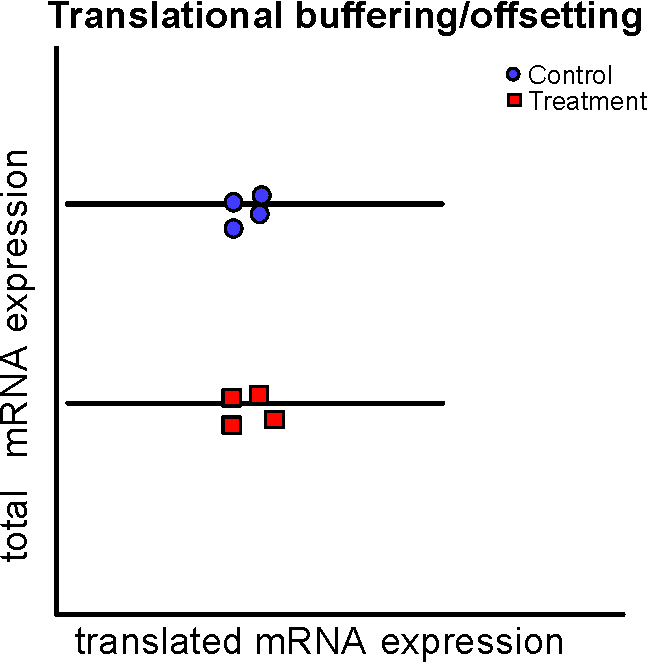
\includegraphics{./figures/geneModes_anota2seq.pdf}
  \caption{anota2seq gene model for analysis of translational buffering /offsetting - Total mRNA expression is set out against translated mRNA expression for each biological replicate and treatment condition. The model shows total mRNA changes that are independent of translated mRNA changes which is classified as translational buffering. It is important to distinguish between the gene modes as their regulation could be due to different underlying biological mechanisms (see section \ref{modes}).
  \label{fig:anota2seq}}
\end{wrapfigure}

Nevertheless, commonly observed in polysome and ribosome profiling data sets are three gene expression modes, translation, translational buffering and mRNA abundance. While anota can be used to identify genes among the translation and mRNA abundance mode, analysis for translational buffering was not implemented therein (\emph{See Figure \ref{fig:anota}}). Therefore, one would need to rely on the integration of several methods to efficiently analyse transcriptome-wide studies of translation efficiences. Anota2seq addresses this issue by changing the analysis model as described in section \ref{algorithm} to analyse changes in total mRNA levels corrected for changes in translated mRNA levels (i.e.~translational buffering, \textbf{see figure \ref{fig:anota2seq}}).

Appliance of anota2seq has successfully identified translational buffering to which biological mechanisms could be linked, e.g.~as mentioned earlier translationally bufferring under ER\(\alpha\) depletion in prostate cancer (\textbf{see section \ref{modeBuffering}}) (Lorent et al., 2019). Furthermore, in \textbf{study 2} translational buffering can be observed as a compensating mechanisms in ``healthy'' cells upon treatment with an eIF4A inhibitor and in \textbf{study 3} we identify mTOR dependent translational buffering for mRNAs with certain 3' UTR characteristics.

The aim of this study is to compare anota2seq's performance to other established algorithms (i.e.~DESeq2, RiboDiff, babel, TE-score and Xtail) for analysis of translation efficiencies, specifically their ability to distinguish the three prominent modes of gene expression. To achieve we used a simulated data based approach. While it is arguable to what extent conclusion drawn from simulated data can be extended towards empirical data it allows for a controlled environment where true positive changes are known in advance. Furthermore, the mean-variance relationship in the simulated data is based on a real polysome profiling data set to increase confidence that drawn conclusions are also applicable to empirical data (Guan et al., 2017).

The simulated data consisted of four replicates for translated mRNA and total mRNA with a ``control'' and a ``treatment'' condition. Furthermore, the data sets contained a combination of the following gene sets:

``Unchanged'': For this simulation category we drew reads from the same NB distribution for both the control and treatment conditions in both the translated and total mRNA. This category represents genes that would be unaffected by e.g.~a stimulus of between cellular states.

``mRNA abundance'': For this category the control condition for both the translated mRNA and total mRNA were drawn from the same NB distribution. The NB distribution for \emph{both translated mRNA and total mRNA} of the treatment condition was altered so that values would be drawn corresponding to a fold change (negative or positive) ranging between 1.5 to 3.0. The directionality of the fold changes (i.e.~up or down regulation) was the same for translated mRNA and total mRNA.

``translation'': For this category the control condition for both the translated mRNA and total mRNA were drawn from the same NB distribution. The NB distribution for \emph{translated mRNA only} of the treatment condition was altered so that values would be drawn corresponding to a fold change (negative or positive) ranging between 1.5 to 3.0.

``buffering'': For this category the control condition for both the translated mRNA and total mRNA were drawn from the same NB distribution. The NB distribution for \emph{total mRNA only} of the treatment condition was altered so that values would be drawn corresponding to a fold change (negative or positive) ranging between 1.5 to 3.0.

As a first step we tested whether the methods could properly control for type-1 errors (i.e.~false positive identification). For this we simulated a data set with genes belonging only to the ``unchanged'' category. This revealed that babel, but to an even greater extent Xtail, were unable to control their type-1 error as these methods assigned low p-values and FDRs when no real changes were present. This indicated a limited applicability of Xtail and babel for statistical analysis of translatomes.

From the comparative analysis of the analysis for changes in translation efficiencies affecting protein levels we concluded that anota2seq outperforms all other methods. This was assessed by comparing the area under the curve from Receiver operating characteristics (ROC) and precision recall curves. The ROC curves showed a, albeit slightly, better performance for detecting changes in translation. However, the precision recall was much higher for anota2seq which can be accredited to that the analysis principle of the other methods is based on identifying changes regardless of whether the change is in the translated mRNA or total mRNA (\emph{as explained in section \ref{algorithm}}). Nevertheless, when comparing the performance using simulated data in the absence of genes belonging to the ``buffering'' category anota2seq still showed superior performance.

Next to the a prior knowledge of the introduced changes in the simulation data, it also allowed us to modify parameters to investigate the robustness of the methods to increased variance, overall sequencing depth and differing sequencing depth between samples. Here, all methods showed robustness against variance and sequencing depth differences between samples as long as a minimum of 5 million counts per sample was reached.

A short coming in the simulation study is that we did not assess the effects of systematic batch effects. Batch effects can be introduced e.g.~during experimental design and there are many methods that try to correct for theseZhang, Parmigiani, \& Johnson (2020). Other ways to correct for batch effects is their inclusion in the analysis model, which can be supplied to the analysis model in DESeq2, edgeR as well as anota2seq. Indeed analysis of a dataset with prominent batch effects showed that batch effects can dampen the efficiency of the anota2seq algorithm to identify changes but can be effectively corrected for in the algorithm.

In this study we developed an analysis algorithm for efficient transcriptome-wide analysis of translation efficiencies applicable to DNA-microarrays and RNA seq. Furthermore, anota2seq has been successfully applied to broaden the knowledge around mRNA translation in various different contexts Chaparro et al. (2020).

\section{Study 2 - eIF4A supports an oncogenic translation program in pancreatic ductal adenocarcinoma}

Pancreatic cancer is considered a lethal malignancy and has limited treatment options. A study on predictions for european cancer mortality rates for 2021 concluded that health efforts should focus on pancreatic cancer. While other cancers (e.g.~ovary, breast and stomach) showed a decline in mortality rates, no major overall decline was observed for pancreatic cancer in the period of 1970-2021 (Carioli et al., 2021).

Pancreatic ductal adeno carcinoma (PDAC) accounts for over 90\% of exocrine pancreatic cancer, whereas non ductal pancreatic cancers e.g.~acinar cell carcinomas are uncommon Jun \& Hong (2016). It is estimated the 60-70\% of the PDACs arise in the head (Luchini, Capelli, \& Scarpa, 2016). So far treatment options are mostly limited to surgical removal, which can be complicated due to the anatomical location of the pancreas head.

With the increasing understanding of tumor heterogeneity, i.e.~tumors with similar tissue origin are not necessarily identical at a molecular level, anti cancer therapy improved (Biankin \& Hudson, 2011). In breast cancer stratification by histological,molecular and gene expression features lead to identification of several breast cancer subtypes for which different treatment options exist, e.g.~\(ER^+\) breast cancer subtypes respond to endocrine therapy whereas \(ER^-\) do notParker et al. (2009). While breast cancer treatment strategies benefit from a rather well established understanding of the molecular subtypes, in pancreatic cancer transcriptomic based subtyping is still ongoing Collisson, Bailey, Chang, \& Biankin (2019). Therefore, it is warranted to extend current knowledge around pancreatic cancer to advance therapeutic strategies in this lethal disease.

While intricacies of molecular subtypes are still being investigated, research has shown that oncogenic mutations in KRAS as well as inactivation of tumor supressors e.g.~TP53 are commonly shared among PDAs (Jones et al., 2008). Furthermore, PDAs have been shown to be dependent on increased protein synthesis mediated by Kras (Chio et al., 2016). This indicates an important role of mRNA translation in PDA.

The aim of \emph{study 2} was to investigate the therapeutic effects of targeting eIF4A in a three dimensional PDA organoid cell culture with mutations in the \(Kras^{LSL-G12D}\), \(Trp53^{LSL-R172H}\) and Pdx1-cre alleles that has been shown to recapitulate PDA tumor progression (Boj et al., 2015). The inhibition of eIF4A was done using a synthetic rocaglate, CR-1-31B (CR-31). Rocaglates have been shown to inhibit eIF4A helicase activity and displayed anti tumor activity (Cencic et al., 2009).

We first wanted to establish the therapeutic validity of targeting eIF4A in PDA. In vitro experiments comparing treated PDA organoids (KP) to their normal (N) counter parts revealed heightened sensitivity of KP to CR-31 treatment. OP-puromycin incorporation showed reduced protein synthesis in KP, whereas N were affected to a lesser extent. Furthermore, similar effects were found in vivo for PDA tumours. Here CR-31 reduced protein synthesis (assessed by SUnSET assay), tumor growth (assessed by ultra sound imaging) and increased survival. The effect on protein synthesis was not due to inhibition of oncogenic signalling pathways which was evaluated western blot assessing the phosphorylation of e.g.~AKT, mTOR and 4E-BP1. From these findings we concluded that there is therapeutic validity in targeting eIF4A in PDA that acts downstream of oncogenic signalling pathways.

Using polysome profiling we then sought to decipher the mechanisms explaining the increased sensitivity to CR-31 in KP organoids. First we investigated the differences in gene expression between untreated KP and N organoids. Analysis of changes in translation efficiencies using anota2seq revealed massive modulation at both transcription and translation indicative of underlying differences in e.g.~genomic stability and enhanced oncogenic signalling impinging on protein synthesis reported in PDA (Boj et al., 2015). Consistent with the in vitro OP-puromycin incorporation and in vivo SUNsET experiments, CR-31 had only little effect on translation in N organoids, whereas in KP organoids exclusively changes in translation were detected.

We then compared the mRNAs affected by CR-31 in KP to the acquired translational profile of untreated KP and N organoids. In order to achieve this we visualised the mRNAs affected by CR-31 in KP onto the data of the untreated KP vs N organoids comparison. This revealed that the acquired translational program of KP organoids is reversed when treated with CR-31.

Performing a similar analysis, we visualised mRNAs sensitive to CR-31 in KP onto the data of the CR-31 treated N organoids. mRNAs affected by CR-31 in KP were translationally buffered in CR-31 treated N organoids. Translational buffering, as an adaptive response to treatment, has been shown to maintain protein homeostasis by inducing a transcriptional response increasing the pool of mRNAs that can be translated (Lorent et al., 2019). The ability for N organoids in increase transcription for mRNAs affected by CR-31, whereas KP cannot, could partially explain as to why protein synthesis is not reduced to a similar extent in N as in KP.

We then assessed 5' UTR characteristics of the translationally regulated mRNAs upon CR-31 treatment in KP organoids. It was reported that eIF4A-senstive mRNAs showed overall and more structured 5' UTRs (e.g.~containing G-quadruplexes) Gandin et al. (2016). Furthermore, a mechanisms by which rocaglates would clamp eIF4A to mRNAs with {[}A,G{]} repeats in their 5 UTR was described (Iwasaki, Floor, \& Ingolia, 2016). However, mRNAs sensitive to CR-31 treatment herein showed overall shorter 5' UTRs that were more structured when corrected for their length without enrichment for 4G-quadruplexes or {[}A,G{]} repeats. From the polysome profiling and UTR analysis we concluded that eIF4A supports an oncogenic translation program in PDA cells for mRNAs with shorter but structured 5' UTRs.

Shorter 5' UTRs have been shown to be sensitive to eIF4E expression and encode for metabolic functions (see section \ref{regmRNA}). When we compared an eIF4E overexpression signature in the KP vs N and CR-31 treated KP we observed that in KP organoids translationally regulated mRNAs under eIF4E overexpression were also translationally activated. This observation is consistent with reports of 4E-BP1 loss in pancreatic cancer (Martineau et al., 2014). eIF4A inhibition in tumors resistant to mTOR inhibiton by loss of 4E-BP1 has been shown to circumvent this resistance (Müller et al., 2019). Indeed, CR-31 treatment in KP reversed the translational profile for eIF4E sensitive mRNAs. Therefore, while rocaglates have been shown to directly target eIF4A (Cencic et al., 2009), eIF4F complex formation could be disrupted by reduced eIF4A availability to an extent that also cap dependent translation is affected in PDA organoids herein.

When further inspecting the regulated gene sets in treated and untreated KP compared to their normal counterparts we could see an enrichment in metabolic pathways, e.g.~Oxidative phosphorylation. This pathway was upregulated in untreated KP compared to N, whereas in KP CR-31 treatment reversed the translational profile of this pathway. Indeed, when we measured mitochondrial respiration (by oxygen consumption rates) we found that CR-31 treatment in KP disrupted this process, whereas N organoids where affected to a lesser extent.

A way to counter loss of energy production through oxidative phosphorylation is to increase activity of other anaerobic metabolic pathways, i.e.~glycolysis. However, in CR-31 treated KP we could not detect a upregulation of glycolysis measured by \(U-C^{13}\) glucose labeling and extra cellular acidification rates nor did CR-31 treatment affect expression of glycolytic enzymes (e.g.~HK1,HK2, LDHA, SLCA1, SLCA3). Furthermore, glucose deprivation did not further sensitise to CR-31 treatment. This was rather unexpected, given that increased glycolysis is characteristic for cancers as described by Otto walburg (Warburg, Wind, \& Negelein, 1927). However, the polysome prolfing data revealed translational downregulation and subsequent reduction of protein expression for the glucose transporter Slc2a6. Indeed, perturbation of Slc2a6 using \(sgRNA^{Slc2a6}\) in N and KP organoids revealed a decrease in glucose uptake. From this we concluded that glycolytic compensation of KP is diminished by translational regulation of the glucose transporter Slc2a6 upon CR-31 treatment.

Among the translationally activated genes in the CR-31 treated KP organoids where mRNAs involved in the glutamine metabolism (i.e.~Slc1a5 and Gls1). Furthermore, glutamine levels were elevated in patient derived PDA cell lines treated with CR-31. Glutamine can be converted into \(\alpha\)-ketoglutarate and funneled into the krebs cycle and therefore can serve to increase energy production (Xiao et al., 2016). Indeed, using gas chromatography mass spectrometry (GC/MS) to quantify metabolites after culturing PDA cells in \(C_5^{13}\)- glutamine, we identified a shift towards reductive carboxylation of \(\alpha\)-ketoglutarate obtained from \(C_5^{13}\)- glutamine to produce acetyl-CoA. Notably, the glutamine metabolism was not elevated in N organoids.

A combined treatment of CR-31 with glutaminase inhibitors (BPTES or CB839) could sensitise to CR-31 treatment patient-derived PDA cells to CR-31 treatment. Therefore, our study suggests an eIF4A dependent translational program in PDA that can act as a theurapeutic target in PDA. Furthermore, a recently published ribosome profiling study of a CR-31 treated human pancreatic cancer cell line (PANC1) observed the same therapeutic effect of CR-31 treatment in vivo on survival and tumor volume (Singh et al., 2021). This underlines the significance of our study in identifying eIF4A as therapeutic target in PDA.

Nevertheless, the same study indicated differences on the underlying regulated mRNA subsets. They report, in line with the literature, that eIF4A depdent mRNAs show long and structured 5' UTRs containing G-quadruplexes Wolfe et al. (2014). While the 5' UTRs of the mRNAs identified herein where overall shorter, they were overall more structured. Furthermore, the mRNAs identifed in Singh et. al.~were involved in KRAS signalling, which was unaltered in our study. Nevertheless, whether G-quadruplexes can actually form stably in cells is still iverstigated. Furthermore, the authors chose to use ribosome profiling in their study that provides nucleotide resolution of ribosome occupancy which could give insights whether ribosomes would stall at such g-quadruplex sites and therefore their possibly their formation. Yet, the authors did not exploit this feature of their applied experimental methodology.

This raises some questions about the differences between experimental setups and their potential influence on biological outcomes and interpretation thereof. For instance, Singh et. al.~performed ribosome profiling on a PANC1 cell line culture treated with 25nM CR-31, wheres herein we performed polysome profiling on a 3D-organoid culture treated with 10nM CR-31. The differences between ribosome and polysome profiling have been discussed extensively (see section \ref{exptMethod}). Furthermore, by measuring IC50 concentrations for CR-31 in a panel of pancreatic cancer cell lines, Singh et. al.~show a \textasciitilde6-fold difference in susceptability to CR-31 between the cell lines of which PANC1 cells were most sensitive to CR-31. Dosage dependent viability experiments of patient derived PDA cells in our study revealed that at 10nM CR-31 treatment cell viability was reduced by \textasciitilde30\%, whereas treatment with 25nM reduced viability by \textgreater{} 50\%. Furthermore, in patient derived PDA a combination treatment of CR-31 and CB839 showed no synergistic effects at 25nM CR-31, whereas at 12.50nM synergy was observed. Therefore, combining the findings of these two studies indicate that CR-31 treatment in PDA indeed has a therapeutic effect, however the underlying mechanisms that are observed in the transcriptome wide analysis of translation efficiencies could be dependent on the experimental method to assess mRNA translation, the model system and treatment dosages.

\section{Study 3 - mTOR-dependent translational buffering overrides transcriptome alterations leading to
maintained proteome composition}

Breast cancer is an umbrella term for a heterogeneous disease with numerous molecular subtypes with different clinical behaviour. Currently, breast cancer is classified into five major groups; luminal A, luminal B, HER-2, basal and normal like. The classification is based on histopatholgy and receptor status. Histopathological are determined by the degree of tumor differentiation (tubule formation), nuclear pleomorphism and proliferation (mitotic count). These features are then scored into a histological grade (I-III) (Eliyatkın, Yalçın, Zengel, Aktaş, \& Vardar, 2015). As mentioned earlier, receptor status of the progesterone (PR), estrogen (ER) and HER-2 are evaluated and have implications for neo adjuvant and adjuvant treatment strategies. Advances in technologies lead to classification of breast cancer subtypes using gene expression profiles,e.g.~the PAM50 classification, that allow for unbiased classification of breast cancer (Parker et al., 2009). A study that correlated the gene expression profiles of the PAM50 classification found a significanlty higher mRNA:protein correlation for PAm50 genes, indicating their prognostic value (Johansson et al., 2019). Nevertheless, the authors observed intermixed luminal B and HER2 clustering based on protein expression in line with the literature that HER2 subtypes receive conflicting mRNA based classifications Prat et al. (2014). Thus, the understanding of breast cancer subtypes has increased tremendously leading to improved and targeted treatment options, however there is need for further research to understand the full breast cancer spectrum on a molecular level.

Another important factor to consider in breast cancer treatment are life style and other health related issues that could impact cancer progression or response to treatment, e.g.~obesity. Studies in the 1970 observed unfavorable prognosis for breast cancer in obese women (Abe, Kumagai, Kimura, Hirosaki, \& Nakamura, 1976). More recent studies observed endocrine therapy to be less effective in obese patients and increased cancer incidence in individuals with higher weight or lack of physical activity Eheman et al. (2012). Obesity can pose an increased risk to develop metabolic disorders such as metabolic syndrome or type 2 diabetes that can lead to hyperinsulinemia, i.e.~elevated physiological insulin levels (Saltiel, 2001).

The role of insulin in the body is to regulate glucose and lipid metabolism as well as protein synthesis. Protein synthesis and metaboloism are often dysregulated in cancer Hanahan \& Weinberg (2011). Insulin can bind to both IGF1R and INSR that activate the PI3K/AKT/mTOR and RAS/ERK signalling pathways. A role of insulin in cancer progression has initially been observed in long term tissues cultures where it increased metabolism as well as growth (Osborne, Bolan, Monaco, \& Lippman, 1976). Another growth factor that is similar to insulin is IGF1 which acts to the same receptors as insulin. IGF1 plays a role in cancer progression and its levels are elevated upon hyperinsulinemia Gallagher \& LeRoith (2010).

The importance of both IGF1 and insulin signalling in cancer has been well established now and led to development of therapeutic strategies by e.g.~targeting both IGF1R and INSR or the PI3K signalling pathway Mayer et al. (2017). Yet, to this day the full extent of insulin signalling on gene expression in cancer has not been established. This study aims to bridge this gap in knowledge by elucidating the effects of insulin signalling on gene expression using a multi-omics (including transcriptomics, translatomics and proteomics) approach to capture multiple steps of the gene expression pathway simultaneously. Furthermore, we asses insulin signalling in cancer cells as well as non-transformed epithelial cells.

We first investigated the effects of insulin on gene expression in a luminal A breast cancer cell line, i.e.~MCF7 cells. Polysome-profiling revealed a strong transcripional and translational response upon insulin stimulation. Among the translationally activated mRNAs were mRNAs with short 5' UTRs that harboured TOP motifs which is n accordance that insulin signalling leads to activation of mTORC1 and phosphorylation of its downstream targets. When visualising the mRNAs in the data where MCF7 cells were stimulated with insulin in the presence of torin1, an mTOR active site inhibitor, we observed that the changes in mRNA translation were almost fully reversed. This led to the conclusion that the effects of insulin on gene expression are to a great extent dependent on mTOR activity.

What was surprising to us was the observation that a subset of mRNAs exhibited translational buffering upon insulin stimulation while mTOR is inhibited. For these mRNAs, the total mRNA levels were increased, whereas the polysome-association was unaltered between conditions effectively uncoupling transcription from translation. As has been seen by others, we confirm that translationally buffered mRNAs maintain constant protein expression across conditions using HiRIEF LC/MS Branca et al. (2014). These finding indicate that mTOR signalling as a gatekeeper for transcriptional programs to fine tune translation in response to extra cellular or intra cellular signals.

MCF7 cells are of epithelial origin and therefore not a ``classical'' insulin sensitive. Their response to insulin prompted us to investigate whether this could be due to cellular plasticity in cancer. To assess this we chose to compare the effects found in MCF7 to a non-malignant epithelial cell type, i.e.~HMEC cells. We found that insulin alone was not sufficient to stimulate the PI3k/AKT/mTOR pathway in HMEC to a similar extent as in MCF7. however, a combination treatment of insulin and IGF1 in HMEC cells elicited a similar reponse as insulin treatment in MCF7 alone. It is known that during hyperinsulinemia IGF1 levels are increased and both IGF1 and insulin signalling has been associated with cancer (Gallagher \& LeRoith, 2010). We therefore opted to compare the combined insulin + IGF1 treatment in HMEC to that of MCF7 assuming their signalling cascades are nearly identical as proposed in the literature Boucher, Tseng, \& Kahn (2010).

Polysome profiling of the insulin + IGF1 stimulated HMEC cells revealed a strong translational response, but was lacking the transcriptional activation found in MCF7 cells. Translationally activated mRNAs in HMEC showed 5' UTR features similar to those in MCF7 cells. Consequently, their translational activation was dependent on mTOR signalling evident from their translational suppression under conditions when mTOR was inhibited during insulin + IGF stimulation. Furthermore, comparing the mRNA signatures of HMEC and MCF7 in the opposite cell line we could observe that changes at the level of translation were in accord across cell types.

In contrast to MCF7 cells, HMEC did not elicit a strong transcriptional response as shown by the small number of changes in mRNA abundance. However, when comparing a recently described transcription signature induced after INSR translocation to the nucleus, we could see that in both HMEC and MCF7 there was a transcriptional response of differing magnitude (Hancock et al., 2019). A possible explanation for the different response in transcription could be due to differences in chromosome instability, exposing DNA to trans acting factors, between the cell lines. While not assessed herein, a transcription factor analysis paired with chromatin immunoprecipitation (ChIP) sequencing could provide insight into this Park (2009). Assuming a consequence of having a weaker transcriptional response, HMEC cells did not elicit translational buffering upon insulin + IGF1 stimulation when mTOR was inhibited. Thus the effects of insulin and IGF1 signalling on mRNA translation are foremost mTOR dependent, however total mRNA responses differ between malignant and non-malignant cells.

The translational buffering in MCF7 prompted us to investigate this phenomenon more. To assess differences dependent on mRNA characteristics we defined two subsets. The ``reversed'' and the ``uncoupled'' (that is translationally buffered when mTOR is inhibited) subsets that only differed in their total mRNA response when mTOR was inhibited during insulin stimulation. To rule out that the observed effects on total mRNA are technical artifacts we validated total mRNA levels for two genes from each subset. The differences in regulation of gene expression were not dependent on codon usage which has been described before in a different context(Lorent et al., 2019). However, overall uncoupled mRNAs had shorter 3' UTRs with a higher GC content and were depleted for HuR binding sites. The depletion of HuR binding sites in the 3' UTRs of the uncoupled subset prompted us to investigate mRNA stability differences. Using a time series experiment under actinomycin D treatment to block transcription quantified using nanoString, we found significant longer mRNA half lifes for the uncoupled subset as compared to the reversed subset. From these data we hypothesised that there are different underlying mechanisms for these subsets that regulate their gene expression under conditions where mRNA translation is dampened. Under this hypothesis the reversed subset is likely regulated through mRNA stability, whereas the more stable uncoupled subset requires to be regulated by translation as their total mRNA level remains high for longer periods of time.

The involvement of HuR in this cannot be fully supported with our current data as the analysis only supports a correlation between the occurrence of HuR binding sites and the 3' UTRs of the reversed subset. The effect on stability could be due to other trans acting factors such as miRNAs (Valinezhad Orang, Safaralizadeh, \& Kazemzadeh-Bavili, 2014). A way to increase confidence is to investigate HuRs involvement experimentally, e.g.~we could use a sgRNA to silence HuR and measure total mRNA levels of the reversed and uncoupled mRNAs previously validated by qPCR. If HuR is involved, we would expect that the reversed mRNAs retain higher total mRNA levels under the condition where mTOR is inhibited during insulin stimulation in MCF7 cells as compared to control. Furthermore, while the differences in total mRNA levels between the insulin and the insulin and torin1 treated conditions in the RNAseq data imply a treatment effect on the mRNA stability we did not observe this in the time chase experiment quantified by nanoString. This raises the question whether the transcription block induced by actinomycin D could influence the regulation of mRNA stability between treatments. We could address this by including actinomycin D in the sgHuR experiment and see if effects thereof differ or an experiment independent of sgHuR. Presence of such an effect could indicate a cross talk between transcription and regulation of mRNA stability.

Since the translational buffering identified herein was only observed in insulin treated cancer cells, we wondered whether this is only specific to this system. Cellular plasticity in cancer allows cancer cells to obtain stem cell like features Quail, Taylor, \& Postovit (2012). Therefore, we reasoned that a system were we study gene expression of stem cells could give some insight whether cancer cells obtained stem cell features that normal epithelial cells do not have. Furthermore, we wanted to investigate whether other means of mTOR inactivation, e.g.~hypoxia, would lead to similar effects on gene expression. To assess these aspects we cultured H9 stem cells in medium with insulin present in normoxia and hypoxia. This experimental setup differs to that of MCF7 and HMEC cells as these were serum starved prior to treatment induction.

Studying this system in H9 we could observe changes for all three modes for regulation of gene expression. Most notably, we observed a large fraction of translationally buffered mRNAs with similar 3' UTR characteristics to that of the uncoupled subset in MCF7 cells. Using publicly available data on mRNA stability we saw that the translationally buffered mRNA were overall more stable as compared to their background. Furthermore, visualising the reversed and uncoupled subset identified in MCF7 in the H9 data we observe differences in their regulation of total mRNA levels, indicating that these subset underlie different regulations even across these two models. Furthermore, these data argue for that translational buffering observed in insulin treated MCF7 cells during mTOR inhibition is not limited to that system but can also occur under more physiological conditions.

Here we present an unprecedented and comprehensive investigation of the effects on insulin on gene expression in cancer cells and non- transformed epithelial cells across multiple steps of the gene expression pathway. Our results indicate that cancer cells have acquired an increased sensitivity to insulin signalling as compared to non-transformed epithelial cells that is largely dependent on mTOR in both cell types. Furthermore, we observed that cancer cells have the ability to translationally buffer mRNAs which is a feature they share with stem cells.

\chapter{Conclusions}

Cancer is a vastly heterogeneous disease that is characterised by uncontrollable growth and proliferation as well as dysregulated metabolism that can evade therapy through acquiring resistance. mRNA translation is a common denominator of these processes and it is therefore paramount to understand the precise mechanisms by which mRNA translation is regulated to better formulate therapeutic strategies against cancer.

This thesis provides an advance in methodology that facilitates transcriptome-wide analysis of translation efficiencies that can be applied to study cancer models and how they adapt to evade therapeutic strategies. Furthermore, by applying this methodology

\hypertarget{acknowledgments}{%
\chapter*{Acknowledgments}\label{acknowledgments}}
\addcontentsline{toc}{chapter}{Acknowledgments}

\hypertarget{references}{%
\chapter*{References}\label{references}}
\addcontentsline{toc}{chapter}{References}

\hypertarget{refs}{}
\begin{CSLReferences}{1}{0}
\leavevmode\hypertarget{ref-Abe1976}{}%
Abe, R., Kumagai, N., Kimura, M., Hirosaki, A., \& Nakamura, T. (1976). Biological characteristics of breast cancer in obesity. \emph{The Tohoku Journal of Experimental Medicine}, \emph{120}(4), 351--359. \url{https://doi.org/10.1620/tjem.120.351}

\leavevmode\hypertarget{ref-Andre2006}{}%
Andre, F., \& Pusztai, L. (2006). Molecular classification of breast cancer: Implications for selection of adjuvant chemotherapy. \emph{Nature Clinical Practice Oncology}, \emph{3}(11), 621--632. \url{https://doi.org/10.1038/ncponc0636}

\leavevmode\hypertarget{ref-Bailey2016}{}%
Bailey, P., Chang, D. K., Nones, K., Johns, A. L., Patch, A.-M., Gingras, M.-C., \ldots{} Grimmond, S. M. (2016). Genomic analyses identify molecular subtypes of pancreatic cancer. \emph{Nature}, \emph{531}(7592), 47--52. \url{https://doi.org/10.1038/nature16965}

\leavevmode\hypertarget{ref-Bailyes1997b}{}%
Bailyes, E. M., Navé, B. T., Soos, M. A., Orr, S. R., Hayward, A. C., \& Siddle, K. (1997). Insulin receptor/{IGF}-{I} receptor hybrids are widely distributed in mammalian tissues: Quantification of individual receptor species by selective immunoprecipitation and immunoblotting. \emph{The Biochemical Journal}, \emph{327 ( Pt 1)}, 209--215. \url{https://doi.org/10.1042/bj3270209}

\leavevmode\hypertarget{ref-Biankin2011}{}%
Biankin, A. V., \& Hudson, T. J. (2011). Somatic variation and cancer: Therapies lost in the mix. \emph{Human Genetics}, \emph{130}(1), 79--91. \url{https://doi.org/10.1007/s00439-011-1010-0}

\leavevmode\hypertarget{ref-Boj2015}{}%
Boj, S. F., Hwang, C.-I., Baker, L. A., Chio, I. I. C., Engle, D. D., Corbo, V., \ldots{} Tuveson, D. A. (2015). Organoid {Models} of {Human} and {Mouse Ductal Pancreatic Cancer}. \emph{Cell}, \emph{160}(1), 324--338. \url{https://doi.org/10.1016/j.cell.2014.12.021}

\leavevmode\hypertarget{ref-Boucher2010}{}%
Boucher, J., Tseng, Y.-H., \& Kahn, C. R. (2010). Insulin and insulin-like growth factor-1 receptors act as ligand-specific amplitude modulators of a common pathway regulating gene transcription. \emph{The Journal of Biological Chemistry}, \emph{285}(22), 17235--17245. \url{https://doi.org/10.1074/jbc.M110.118620}

\leavevmode\hypertarget{ref-Branca2014}{}%
Branca, R. M. M., Orre, L. M., Johansson, H. J., Granholm, V., Huss, M., Pérez-Bercoff, Å., \ldots{} Lehtiö, J. (2014). {HiRIEF LC}-{MS} enables deep proteome coverage and unbiased proteogenomics. \emph{Nature Methods}, \emph{11}(1), 59--62. \url{https://doi.org/10.1038/nmeth.2732}

\leavevmode\hypertarget{ref-Carioli2021}{}%
Carioli, G., Malvezzi, M., Bertuccio, P., Boffetta, P., Levi, F., Vecchia, C. L., \& Negri, E. (2021). European cancer mortality predictions for the year 2021 with focus on pancreatic and female lung cancer. \emph{Annals of Oncology}, \emph{0}(0). \url{https://doi.org/10.1016/j.annonc.2021.01.006}

\leavevmode\hypertarget{ref-Cencic2009}{}%
Cencic, R., Carrier, M., Galicia-Vázquez, G., Bordeleau, M.-E., Sukarieh, R., Bourdeau, A., \ldots{} Pelletier, J. (2009). Antitumor {Activity} and {Mechanism} of {Action} of the {Cyclopenta}{[}b{]}benzofuran, {Silvestrol}. \emph{PLoS ONE}, \emph{4}(4). \url{https://doi.org/10.1371/journal.pone.0005223}

\leavevmode\hypertarget{ref-Chan2019}{}%
Chan, K., Robert, F., Oertlin, C., Kapeller-Libermann, D., Avizonis, D., Gutierrez, J., \ldots{} Chio, I. I. C. (2019). {eIF4A} supports an oncogenic translation program in pancreatic ductal adenocarcinoma. \emph{Nature Communications}, \emph{10}(1), 5151. \url{https://doi.org/10.1038/s41467-019-13086-5}

\leavevmode\hypertarget{ref-Chaparro2020}{}%
Chaparro, V., Leroux, L.-P., Masvidal, L., Lorent, J., Graber, T. E., Zimmermann, A., \ldots{} Jaramillo, M. (2020). Translational profiling of macrophages infected with {Leishmania} donovani identifies {mTOR}- and {eIF4A}-sensitive immune-related transcripts. \emph{PLOS Pathogens}, \emph{16}(6), e1008291. \url{https://doi.org/10.1371/journal.ppat.1008291}

\leavevmode\hypertarget{ref-Chio2016}{}%
Chio, I. I. C., Jafarnejad, S. M., Ponz-Sarvise, M., Park, Y., Rivera, K., Palm, W., \ldots{} Tuveson, D. A. (2016). {NRF2 Promotes Tumor Maintenance} by {Modulating mRNA Translation} in {Pancreatic Cancer}. \emph{Cell}, \emph{166}(4), 963--976. \url{https://doi.org/10.1016/j.cell.2016.06.056}

\leavevmode\hypertarget{ref-Christopoulos2015}{}%
Christopoulos, P. F., Msaouel, P., \& Koutsilieris, M. (2015). The role of the insulin-like growth factor-1 system in breast cancer. \emph{Molecular Cancer}, \emph{14}(1), 43. \url{https://doi.org/10.1186/s12943-015-0291-7}

\leavevmode\hypertarget{ref-Collisson2019}{}%
Collisson, E. A., Bailey, P., Chang, D. K., \& Biankin, A. V. (2019). Molecular subtypes of pancreatic cancer. \emph{Nature Reviews Gastroenterology \& Hepatology}, \emph{16}(4), 207--220. \url{https://doi.org/10.1038/s41575-019-0109-y}

\leavevmode\hypertarget{ref-Collisson2011}{}%
Collisson, E. A., Sadanandam, A., Olson, P., Gibb, W. J., Truitt, M., Gu, S., \ldots{} Gray, J. W. (2011). Subtypes of pancreatic ductal adenocarcinoma and their differing responses to therapy. \emph{Nature Medicine}, \emph{17}(4), 500--503. \url{https://doi.org/10.1038/nm.2344}

\leavevmode\hypertarget{ref-Eheman2012}{}%
Eheman, C., Henley, S. J., Ballard-Barbash, R., Jacobs, E. J., Schymura, M. J., Noone, A.-M., \ldots{} Edwards, B. K. (2012). Annual {Report} to the {Nation} on the status of cancer, 1975-2008, featuring cancers associated with excess weight and lack of sufficient physical activity. \emph{Cancer}, \emph{118}(9), 2338--2366. \url{https://doi.org/10.1002/cncr.27514}

\leavevmode\hypertarget{ref-Eliyatkin2015}{}%
Eliyatkın, N., Yalçın, E., Zengel, B., Aktaş, S., \& Vardar, E. (2015). Molecular {Classification} of {Breast Carcinoma}: {From Traditional}, {Old}-{Fashioned Way} to {A New Age}, and {A New Way}. \emph{The Journal of Breast Health}, \emph{11}(2), 59--66. \url{https://doi.org/10.5152/tjbh.2015.1669}

\leavevmode\hypertarget{ref-Feldmann2007}{}%
Feldmann, G., Beaty, R., Hruban, R. H., \& Maitra, A. (2007). Molecular genetics of pancreatic intraepithelial neoplasia. \emph{Journal of Hepato-Biliary-Pancreatic Surgery}, \emph{14}(3), 224--232. \url{https://doi.org/10.1007/s00534-006-1166-5}

\leavevmode\hypertarget{ref-Gallagher2010}{}%
Gallagher, E. J., \& LeRoith, D. (2010). The {Proliferating Role} of {Insulin} and {Insulin}-{Like Growth Factors} in {Cancer}. \emph{Trends in Endocrinology and Metabolism: TEM}, \emph{21}(10), 610--618. \url{https://doi.org/10.1016/j.tem.2010.06.007}

\leavevmode\hypertarget{ref-Gandin2016a}{}%
Gandin, V., Masvidal, L., Hulea, L., Gravel, S.-P., Cargnello, M., McLaughlan, S., \ldots{} Topisirovic, I. (2016). {nanoCAGE} reveals 5' {UTR} features that define specific modes of translation of functionally related {MTOR}-sensitive {mRNAs}. \emph{Genome Research}, \emph{26}(5), 636--648. \url{https://doi.org/10.1101/gr.197566.115}

\leavevmode\hypertarget{ref-Guan2017}{}%
Guan, B.-J., van Hoef, V., Jobava, R., Elroy-Stein, O., Valasek, L. S., Cargnello, M., \ldots{} Hatzoglou, M. (2017). A {Unique ISR Program Determines Cellular Responses} to {Chronic Stress}. \emph{Molecular Cell}, \emph{68}(5), 885--900.e6. \url{https://doi.org/10.1016/j.molcel.2017.11.007}

\leavevmode\hypertarget{ref-Hanahan2011}{}%
Hanahan, D., \& Weinberg, R. A. (2011). Hallmarks of cancer: {The} next generation. \emph{Cell}, \emph{144}(5), 646--674. \url{https://doi.org/10.1016/j.cell.2011.02.013}

\leavevmode\hypertarget{ref-Hancock2019}{}%
Hancock, M. L., Meyer, R. C., Mistry, M., Khetani, R. S., Wagschal, A., Shin, T., \ldots{} Flanagan, J. G. (2019). Insulin {Receptor Associates} with {Promoters Genome}-wide and {Regulates Gene Expression}. \emph{Cell}, \emph{177}(3), 722--736.e22. \url{https://doi.org/10.1016/j.cell.2019.02.030}

\leavevmode\hypertarget{ref-Hipolito2019}{}%
Hipolito, V. E. B., Diaz, J. A., Tandoc, K. V., Oertlin, C., Ristau, J., Chauhan, N., \ldots{} Botelho, R. J. (2019). Enhanced translation expands the endo-lysosome size and promotes antigen presentation during phagocyte activation. \emph{PLOS Biology}, \emph{17}(12), e3000535. \url{https://doi.org/10.1371/journal.pbio.3000535}

\leavevmode\hypertarget{ref-Iwasaki2016}{}%
Iwasaki, S., Floor, S. N., \& Ingolia, N. T. (2016). Rocaglates convert {DEAD}-box protein {eIF4A} into a sequence-selective translational repressor. \emph{Nature}, \emph{534}(7608), 558--561. \url{https://doi.org/10.1038/nature17978}

\leavevmode\hypertarget{ref-Jewer2020b}{}%
Jewer, M., Lee, L., Leibovitch, M., Zhang, G., Liu, J., Findlay, S. D., \ldots{} Postovit, L.-M. (2020). Translational control of breast cancer plasticity. \emph{Nature Communications}, \emph{11}(1), 2498. \url{https://doi.org/10.1038/s41467-020-16352-z}

\leavevmode\hypertarget{ref-Johansson2019}{}%
Johansson, H. J., Socciarelli, F., Vacanti, N. M., Haugen, M. H., Zhu, Y., Siavelis, I., \ldots{} Lehtiö, J. (2019). Breast cancer quantitative proteome and proteogenomic landscape. \emph{Nature Communications}, \emph{10}(1), 1600. \url{https://doi.org/10.1038/s41467-019-09018-y}

\leavevmode\hypertarget{ref-Johnson2007}{}%
Johnson, W. E., Li, C., \& Rabinovic, A. (2007). Adjusting batch effects in microarray expression data using empirical {Bayes} methods. \emph{Biostatistics (Oxford, England)}, \emph{8}(1), 118--127. \url{https://doi.org/10.1093/biostatistics/kxj037}

\leavevmode\hypertarget{ref-Jones2008}{}%
Jones, S., Zhang, X., Parsons, D. W., Lin, J. C.-H., Leary, R. J., Angenendt, P., \ldots{} Kinzler, K. W. (2008). Core {Signaling Pathways} in {Human Pancreatic Cancers Revealed} by {Global Genomic Analyses}. \emph{Science}, \emph{321}(5897), 1801--1806. \url{https://doi.org/10.1126/science.1164368}

\leavevmode\hypertarget{ref-Jun2016}{}%
Jun, S.-Y., \& Hong, S.-M. (2016). Nonductal {Pancreatic Cancers}. \emph{Surgical Pathology Clinics}, \emph{9}(4), 581--593. \url{https://doi.org/10.1016/j.path.2016.05.005}

\leavevmode\hypertarget{ref-Kuijjer2013}{}%
Kuijjer, M. L., Peterse, E. F., van den Akker, B. E., Briaire-de Bruijn, I. H., Serra, M., Meza-Zepeda, L. A., \ldots{} Cleton-Jansen, A.-M. (2013). {IR}/{IGF1R} signaling as potential target for treatment of high-grade osteosarcoma. \emph{BMC Cancer}, \emph{13}(1), 245. \url{https://doi.org/10.1186/1471-2407-13-245}

\leavevmode\hypertarget{ref-Larsson2010}{}%
Larsson, O., Sonenberg, N., \& Nadon, R. (2010). Identification of differential translation in genome wide studies. \emph{Proceedings of the National Academy of Sciences}, \emph{107}(50), 21487--21492. \url{https://doi.org/10.1073/pnas.1006821107}

\leavevmode\hypertarget{ref-Larsson2011}{}%
Larsson, O., Sonenberg, N., \& Nadon, R. (2011). Anota: {Analysis} of differential translation in genome-wide studies. \emph{Bioinformatics (Oxford, England)}, \emph{27}(10), 1440--1441. \url{https://doi.org/10.1093/bioinformatics/btr146}

\leavevmode\hypertarget{ref-Law2014}{}%
Law, C. W., Chen, Y., Shi, W., \& Smyth, G. K. (2014). Voom: Precision weights unlock linear model analysis tools for {RNA}-seq read counts. \emph{Genome Biology}, \emph{15}(2), R29. \url{https://doi.org/10.1186/gb-2014-15-2-r29}

\leavevmode\hypertarget{ref-Lee2019}{}%
Lee, K., Kruper, L., Dieli-Conwright, C. M., \& Mortimer, J. E. (2019). The {Impact} of {Obesity} on {Breast Cancer Diagnosis} and {Treatment}. \emph{Current Oncology Reports}, \emph{21}(5). \url{https://doi.org/10.1007/s11912-019-0787-1}

\leavevmode\hypertarget{ref-Leek2014}{}%
Leek, J. T. (2014). Svaseq: Removing batch effects and other unwanted noise from sequencing data. \emph{Nucleic Acids Research}, \emph{42}(21), e161--e161. \url{https://doi.org/10.1093/nar/gku864}

\leavevmode\hypertarget{ref-Lorent2019}{}%
Lorent, J., Kusnadi, E. P., van Hoef, V., Rebello, R. J., Leibovitch, M., Ristau, J., \ldots{} Furic, L. (2019). Translational offsetting as a mode of estrogen receptor {\(\alpha\)}-dependent regulation of gene~expression. \emph{The EMBO Journal}, \emph{38}(23), e101323. \url{https://doi.org/10.15252/embj.2018101323}

\leavevmode\hypertarget{ref-Love2014}{}%
Love, M. I., Huber, W., \& Anders, S. (2014). Moderated estimation of fold change and dispersion for {RNA}-seq data with {DESeq2}. \emph{Genome Biology}, \emph{15}(12), 550. \url{https://doi.org/10.1186/s13059-014-0550-8}

\leavevmode\hypertarget{ref-Luchini2016}{}%
Luchini, C., Capelli, P., \& Scarpa, A. (2016). Pancreatic {Ductal Adenocarcinoma} and {Its Variants}. \emph{Surgical Pathology Clinics}, \emph{9}(4), 547--560. \url{https://doi.org/10.1016/j.path.2016.05.003}

\leavevmode\hypertarget{ref-Martineau2014}{}%
Martineau, Y., Azar, R., Müller, D., Lasfargues, C., El Khawand, S., Anesia, R., \ldots{} Pyronnet, S. (2014). Pancreatic tumours escape from translational control through {4E}-{BP1} loss. \emph{Oncogene}, \emph{33}(11), 1367--1374. \url{https://doi.org/10.1038/onc.2013.100}

\leavevmode\hypertarget{ref-Mayer2017}{}%
Mayer, I. A., Abramson, V. G., Formisano, L., Balko, J. M., Estrada, M. V., Sanders, M. E., \ldots{} Arteaga, C. L. (2017). A {Phase Ib Study} of {Alpelisib} ({BYL719}), a {PI3K\(\alpha\)}-{Specific Inhibitor}, with {Letrozole} in {ER}+/{HER2}- {Metastatic Breast Cancer}. \emph{Clinical Cancer Research: An Official Journal of the American Association for Cancer Research}, \emph{23}(1), 26--34. \url{https://doi.org/10.1158/1078-0432.CCR-16-0134}

\leavevmode\hypertarget{ref-Moffitt2015}{}%
Moffitt, R. A., Marayati, R., Flate, E. L., Volmar, K. E., Loeza, S. G. H., Hoadley, K. A., \ldots{} Yeh, J. J. (2015). Virtual microdissection identifies distinct tumor- and stroma-specific subtypes of pancreatic ductal adenocarcinoma. \emph{Nature Genetics}, \emph{47}(10), 1168--1178. \url{https://doi.org/10.1038/ng.3398}

\leavevmode\hypertarget{ref-Molinaro2019a}{}%
Molinaro, A., Becattini, B., Mazzoli, A., Bleve, A., Radici, L., Maxvall, I., \ldots{} Solinas, G. (2019). Insulin-{Driven PI3K}-{AKT Signaling} in the {Hepatocyte Is Mediated} by {Redundant PI3K\(\alpha\)} and {PI3K\(\beta\) Activities} and {Is Promoted} by {RAS}. \emph{Cell Metabolism}, \emph{29}(6), 1400--1409.e5. \url{https://doi.org/10.1016/j.cmet.2019.03.010}

\leavevmode\hypertarget{ref-Muller2019}{}%
Müller, D., Shin, S., Goullet de Rugy, T., Samain, R., Baer, R., Strehaiano, M., \ldots{} Martineau, Y. (2019). {eIF4A} inhibition circumvents uncontrolled {DNA} replication mediated by {4E}-{BP1} loss in pancreatic cancer. \emph{JCI Insight}, \emph{4}(21). \url{https://doi.org/10.1172/jci.insight.121951}

\leavevmode\hypertarget{ref-Osborne1976}{}%
Osborne, C. K., Bolan, G., Monaco, M. E., \& Lippman, M. E. (1976). Hormone responsive human breast cancer in long-term tissue culture: Effect of insulin. \emph{Proceedings of the National Academy of Sciences of the United States of America}, \emph{73}(12), 4536--4540.

\leavevmode\hypertarget{ref-Park2009}{}%
Park, P. J. (2009). {ChIP}{}seq: Advantages and challenges of a maturing technology. \emph{Nature Reviews Genetics}, \emph{10}(10), 669--680. \url{https://doi.org/10.1038/nrg2641}

\leavevmode\hypertarget{ref-Parker2009}{}%
Parker, J. S., Mullins, M., Cheang, M. C. U., Leung, S., Voduc, D., Vickery, T., \ldots{} Bernard, P. S. (2009). Supervised {Risk Predictor} of {Breast Cancer Based} on {Intrinsic Subtypes}. \emph{Journal of Clinical Oncology}, \emph{27}(8), 1160--1167. \url{https://doi.org/10.1200/JCO.2008.18.1370}

\leavevmode\hypertarget{ref-Pollak2008}{}%
Pollak, M. (2008). Insulin and insulin-like growth factor signalling in neoplasia. \emph{Nature Reviews Cancer}, \emph{8}(12), 915--928. \url{https://doi.org/10.1038/nrc2536}

\leavevmode\hypertarget{ref-Prat2014}{}%
Prat, A., Carey, L. A., Adamo, B., Vidal, M., Tabernero, J., Cortés, J., \ldots{} Baselga, J. (2014). Molecular features and survival outcomes of the intrinsic subtypes within {HER2}-positive breast cancer. \emph{Journal of the National Cancer Institute}, \emph{106}(8). \url{https://doi.org/10.1093/jnci/dju152}

\leavevmode\hypertarget{ref-Puleo2018}{}%
Puleo, F., Nicolle, R., Blum, Y., Cros, J., Marisa, L., Demetter, P., \ldots{} Maréchal, R. (2018). Stratification of {Pancreatic Ductal Adenocarcinomas Based} on {Tumor} and {Microenvironment Features}. \emph{Gastroenterology}, \emph{155}(6), 1999--2013.e3. \url{https://doi.org/10.1053/j.gastro.2018.08.033}

\leavevmode\hypertarget{ref-Quail2012}{}%
Quail, D. F., Taylor, M. J., \& Postovit, L.-M. (2012). Microenvironmental regulation of cancer stem cell phenotypes. \emph{Current Stem Cell Research \& Therapy}, \emph{7}(3), 197--216. \url{https://doi.org/10.2174/157488812799859838}

\leavevmode\hypertarget{ref-Rubio2014}{}%
Rubio, C. A., Weisburd, B., Holderfield, M., Arias, C., Fang, E., DeRisi, J. L., \& Fanidi, A. (2014). Transcriptome-wide characterization of the {eIF4A} signature highlights plasticity in translation regulation. \emph{Genome Biology}, \emph{15}(10), 476. \url{https://doi.org/10.1186/s13059-014-0476-1}

\leavevmode\hypertarget{ref-Saltiel2001}{}%
Saltiel, A. R. (2001). New {Perspectives} into the {Molecular Pathogenesis} and {Treatment} of {Type} 2 {Diabetes}. \emph{Cell}, \emph{104}(4), 517--529. \url{https://doi.org/10.1016/S0092-8674(01)00239-2}

\leavevmode\hypertarget{ref-Singh2021}{}%
Singh, K., Lin, J., Lecomte, N., Mohan, P., Gokce, A., Sanghvi, V. R., \ldots{} Wendel, H.-G. (2021). Targeting {eIF4A Dependent Translation} of {KRAS Signaling Molecules}. \emph{Cancer Research}. \url{https://doi.org/10.1158/0008-5472.CAN-20-2929}

\leavevmode\hypertarget{ref-Solomon1988}{}%
Solomon, M. J., Larsen, P. L., \& Varshavsky, A. (1988). Mapping protein-{DNA} interactions in vivo with formaldehyde: Evidence that histone {H4} is retained on a highly transcribed gene. \emph{Cell}, \emph{53}(6), 937--947. \url{https://doi.org/10.1016/s0092-8674(88)90469-2}

\leavevmode\hypertarget{ref-Tebaldi2014}{}%
Tebaldi, T., Dassi, E., Kostoska, G., Viero, G., \& Quattrone, A. (2014). {tRanslatome}: An {R}/{Bioconductor} package to portray translational control. \emph{Bioinformatics}, \emph{30}(2), 289--291. \url{https://doi.org/10.1093/bioinformatics/btt634}

\leavevmode\hypertarget{ref-Tebaldi2012}{}%
Tebaldi, T., Re, A., Viero, G., Pegoretti, I., Passerini, A., Blanzieri, E., \& Quattrone, A. (2012). Widespread uncoupling between transcriptome and translatome variations after a stimulus in mammalian cells. \emph{BMC Genomics}, \emph{13}(1), 220. \url{https://doi.org/10.1186/1471-2164-13-220}

\leavevmode\hypertarget{ref-ValinezhadOrang2014}{}%
Valinezhad Orang, A., Safaralizadeh, R., \& Kazemzadeh-Bavili, M. (2014). Mechanisms of {miRNA}-{Mediated Gene Regulation} from {Common Downregulation} to {mRNA}-{Specific Upregulation}. \emph{International Journal of Genomics}, \emph{2014}. \url{https://doi.org/10.1155/2014/970607}

\leavevmode\hypertarget{ref-Wahl2017}{}%
Wahl, G. M., \& Spike, B. T. (2017). Cell state plasticity, stem cells, {EMT}, and the generation of intra-tumoral heterogeneity. \emph{NPJ Breast Cancer}, \emph{3}, 14. \url{https://doi.org/10.1038/s41523-017-0012-z}

\leavevmode\hypertarget{ref-Warburg1927}{}%
Warburg, O., Wind, F., \& Negelein, E. (1927). {THE METABOLISM OF TUMORS IN THE BODY}. \emph{The Journal of General Physiology}, \emph{8}(6), 519--530. \url{https://doi.org/10.1085/jgp.8.6.519}

\leavevmode\hypertarget{ref-Wolfe2014}{}%
Wolfe, A. L., Singh, K., Zhong, Y., Drewe, P., Rajasekhar, V. K., Sanghvi, V. R., \ldots{} Wendel, H.-G. (2014). {RNA G}-quadruplexes cause {eIF4A}-dependent oncogene translation in cancer. \emph{Nature}, \emph{513}(7516), 65--70. \url{https://doi.org/10.1038/nature13485}

\leavevmode\hypertarget{ref-Xiao2016a}{}%
Xiao, D., Zeng, L., Yao, K., Kong, X., Wu, G., \& Yin, Y. (2016). The glutamine-alpha-ketoglutarate ({AKG}) metabolism and its nutritional implications. \emph{Amino Acids}, \emph{48}(9), 2067--2080. \url{https://doi.org/10.1007/s00726-016-2254-8}

\leavevmode\hypertarget{ref-Zhang2020}{}%
Zhang, Y., Parmigiani, G., \& Johnson, W. E. (2020). {ComBat}-seq: Batch effect adjustment for {RNA}-seq count data. \emph{NAR Genomics and Bioinformatics}, \emph{2}(lqaa078). \url{https://doi.org/10.1093/nargab/lqaa078}

\end{CSLReferences}

\end{document}
